\chapter{Text bearbeiten mit dem "`WYSIWYG"' Editor}
\label{sec:editor}

"`WYSIWYG"' steht für "`What you see is what you get"',  also dass man schon bei der Eingabe sieht wie der Text letztendlich aussehen wird.

Die angezeigten Formatierungs-Möglichkeiten können sich je nach Konfiguration und Editor-Version von Ihrer Installation unterscheiden.

\begin{figure}[htp]
\centering
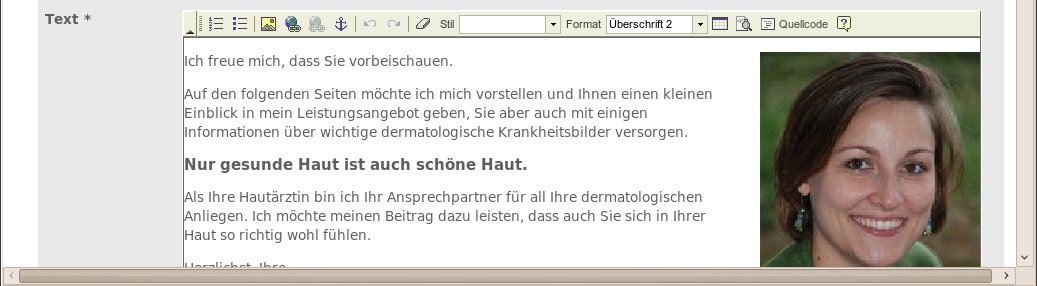
\includegraphics[width=0.9\textwidth]{../../../ullCorePlugin/doc/manual/figures/editor}
\caption{WYSIWYG-Editor}
\label{fig:editor}
\end{figure}

\section{Text schreiben}

Geben Sie wie von anderen Texteditoren gewohnt den Text ein.

Tipp: $\Enter$ erzeugt einen neuen Paragrafen, also einen Textblock mit einer Leerzeile dahinter. Einen einfachen Zeilenumbruch erreichen Sie mit $\Shift + \Enter$.

\section{Text formatieren}

Markieren Sie den gewünschten Text und wählen Sie aus der Editor-Menüleiste die gewünschte Auszeichnung.

Bitte beachten Sie, dass die von uns ausgewählten
Formatierungsmöglichkeiten nach semantischen Gesichtspunkten ausgewählt
wurden. Sie finden also nur „logische“ Auszeichnungen wie zum Beispiel
„wichtig“ oder „Überschrift“, und keine rein optischen
Formatierungsmöglichkeiten wie Farben oder Schriftgrößen. Somit werden
saubere und zukunftssichere Texte gewährleistet. (Stichwort "`semantic
Web"')

Die wichtigsten Formatierungen (von links nach rechts):

\begin{itemize}
\item Nummerierte Liste
\item Liste mit Aufzählungszeichen
\item Stile: "`Important"' -- also "`Wichtig"' wird fett angezeigt
\item Format: "`Überschrift"'
\end{itemize}


\section{Bild einfügen}

\begin{itemize}
\item Setzten Sie den Cursor an die gewünschte Stelle im Text
\item Klicken Sie auf das Bildsymbol 
\includegraphics[height=5mm]{../../../ullCorePlugin/doc/manual/figures/image_icon}
\item Wählen Sie "`Server durchsuchen"'
\item Wählen oder erstellen Sie gegebenenfalls einen neuen Ordner um eine ordentliche Struktur Ihrer Daten zu gewährleisten
\item Wenn Sie ein neues Bild hochladen möchten klicken Sie auf "`Durchsuchen"' und wählen Sie eine Bilddatei von Ihrem Computer aus.
\item Vergessen Sie nicht danach auf "`Upload"' zu klicken
\item Wählen Sie nun ein Bild aus der Liste durch anklicken.
\item Klicken Sie auf "`OK"'
\end{itemize}

\section{Bildeigenschaften ändern}

Klicken Sie mit der rechten Maustaste auf das Bild und wählen Sie "`Bildeigenschaften"'.

Im folgenden werden die wichtigsten Eigenschaften erklärt:

\subsection{Reiter "`Bild-Info"'}

\begin{itemize}
\item Breite / Höhe - Wählen Sie die gewünschte Größe des Bildes in Pixel. Bitte beachten Sie, dass Bilder bereits vor dem Hochladen mit einem Grafikprogramm auf die endgültige Größe skaliert werden sollten
\item Ausrichtung - Wählen Sie "`Links"' oder "`Rechts"' wenn der Text das Bild umfließen soll.
\end{itemize}

\subsection{Reiter "`Erweitert"'}

Wenn Sie das Bild vom Text umfließen lassen ist häufig auf gewissen Seiten des Bildes ein Abstand erwünscht.
Dieser Abstand kann im Feld "`Style"' angegeben werden. Beispiel für einen Abstand links und unten: "`margin-left: 1.5em; margin-bottom: 1.5em;"'


\section{Link erstellen}

Normale Webadressen und E-Mailadressen werden in der normalen Ansicht für die Besucher der Webseite automatisch verlinkt.

Beispiele:

\begin{itemize}
\item www.ullright.org
\item http://ull.at
\item office@ull.at
\end{itemize}

Möchten Sie hingegen gewisse Wörter im Text verlinken markieren Sie die Wörter und klicken Sie auf das Linksymbol 
\includegraphics[height=5mm]{../../../ullCorePlugin/doc/manual/figures/link_icon} (blau-grüne Erdkugel).

\subsection{Link zu einer Internetadresse (URL)}
Geben Sie bei "`URL"' die gewünschte Adresse ein. Beispiel: \url{http://www.ullright.org}

Bei Links zu Internetseiten empfiehlt sich die Seite in einem neuen Browserfenster zu öffnen. Wählen Sie hierzu im Reiter "`Zielseite"' "`Neues Fenster (\_blank)"'.

Zusätzlich empfehlen wir einen solchen Link durch das Symbol für "`Externe Seite"' zu kennzeichen. Schreiben Sie dazu im Reiter "`Erweitert"' die Anweisung "`link\_external"' in das Feld "`Stylesheet Klasse"'.

\subsection{Link zu einer anderen CMS-Seite}

Öffnen Sie die Zielseite in einem neuen Browsertab oder -fenster und kopieren Sie die URL aus der Adressleiste.

Beispiel: \url{http://www.ull.at/ullCms/show/kontakt}

Geben Sie nun bei "`URL"' die gekürzte Adresse startend mit den Schrägstrich nach dem Domänennamen ein.

Beispiel: \url{/ullCms/show/kontakt}

\subsection{E-Mail Link}

Wählen Sie bei "`Link-Typ"' E-Mail und geben Sie die gewünschte E-Mailadresse ein.



\section{Datei hochladen}
\label{sec:upload_file}

Das Hochladen einer Datei funktioniert wie eine Mischung aus Link- und Bildeinfügen.

\begin{itemize}
\item Markieren Sie die Wörter die mit der Datei verlinkt werden sollen
\item Klicken Sie auf das Linksymbol 
\includegraphics[height=5mm]{../../../ullCorePlugin/doc/manual/figures/link_icon}
\item Wählen Sie „Server durchsuchen“
\item Wählen oder erstellen Sie gegebenenfalls einen neuen Ordner um eine ordentliche Struktur Ihrer Daten zu gewährleisten
\item Wenn Sie eine neue Datei hochladen möchten klicken Sie auf "`Durchsuchen"' und wählen Sie eine Datei von Ihrem Computer aus
\item Vergessen Sie nicht danach auf "`Upload"' zu klicken
\item Wählen Sie nun die Datei aus der Liste durch anklicken
\item Klicken Sie auf "`OK"'
\end{itemize}


\section{Tip für PDF-Dateien}

Auf vielen PCs wird bei einem Klick auf den Link zu einer PDF-Datei das PDF direkt im Browserfenster geöffnet. Besuchern passiert es dann häufig, dass sie nach dem Lesen das Fenster oder Tab einfach schließen, und somit auch Ihre Website verlassen.

Um diesem unerwünschten Verhalten vorzubeugen empfiehlt sich ein PDF in einem Pop-up Fenster zu öffnen:

\begin{itemize}
\item Verlinken Sie eine PDF-Datei wie im Kapitel \vref{sec:upload_file} beschrieben
\item Klicken Sie mit der rechten Maustaste auf den Link zur PDF-Datei und wählen Sie "`Link editieren"'
\item Im Reiter "`Zielseite"' wählen Sie nun "`Pop-up Fenster"'
\item Haken Sie die Felder "`Vergrößerbar"', "`Adress-Leiste"', "`Menüleiste"' und "`Rollbalken"' an.
\item Schließen Sie den Vorgang mit "`OK"' ab.
\end{itemize}